\pgfplotstablegetelem{\thepart}{[index]\columnIndex}\of{\cronograma}
\part{\pgfplotsretval}
\label{part:\thepart}
\frame{\partpage}


\begin{frame}[t]{Exemplos de criação de classe}
	
	\fontsize{14pt}{15}\selectfont{
		
		...continuando a partir da aula passada sobre \gls{poo}.
		
	}\par
	\vspace{1em}
	
	
\end{frame}





\begin{frame}[t]{Exercícios}
	\fontsize{10pt}{15}\selectfont{
		Escreva o algoritmo e programa. Use Herança de \gls{poo} para resolver.
		\begin{itemize}%[<+->]
			\item \glsfirst{exercicio_018}: \glsdesc{exercicio_018}
			\vspace{0.5em}
			%			
\includegraphics[scale=0.06]{imagens/fig-atencao-pessoas-estudando.png}
		\end{itemize}
	}\par
	\vspace{1em}
\end{frame}


\begin{frame}[t]{Algoritmo}
	\fontsize{9pt}{9}\selectfont{
		\begin{itemize}%[<+->]
			\item Ler quantidade atual (qtd\_atual) quantidade máxima (qtd\_max) e quantidade mínima em estoque (qtd\_min).
			\item Obtenha a quantidade média do estoque, dado por qtd\_media = (qtd\_max + qtd\_min)/2.
			\item Obtenha a quantidade média do estoque crítico, dado por qtd\_media\_critico = (qtd\_max - qtd\_min)/2.
			\item Obtenha a situação do estoque, dada por\\ 
			situacao\_estoque = Se qtd\_atual >= qtd\_media, então 'Não efetuar compra' SeNão 'Efetuar compra'
			\item Obtenha a situação do estoque crítico, dada por\\ 
			situacao\_estoque\_critico = Se qtd\_atual >= qtd\_media\_critico, então 'Não efetuar compra' SeNão 'Efetuar compra'
			\item Escreva a quantidade média do estoque qtd\_media.
			\item Escreva a quantidade média do estoque crítico qtd\_media\_critico.
			\item Escreva a situação do estoque
			\item Escreva a situação do estoque crítico
		\end{itemize}
	}\par
	\vspace{0.5em}
	Exemplo:\\
	entradas de dados 220,400 e 50.\\
	Saídas\\
	quantidade média do estoque: 225\\
	quantidade média do estoque: 175\\
	situação do estoque: Efetuar compra \# 400+50=450, 450/2=225, 220>=225, SeNão... \\
	situação do estoque crítico: Não efetuar compra \# 400-50=350, 350/2=175, 220>=175, então...
	
\end{frame}




\begin{frame}[t]{Solução do exercício}
	
	\vspace{-0.5em}
	
	\centering
	\makebox[\linewidth][c]{
		\begin{minipage}{0.95\textwidth}
			\inputminted[fontsize={\fontsize{7}{7}\selectfont}]{python}{outros/codigos/python/exemplos-de-aulas/src/codigo_020_classe_estoque_e_estoque_critico.py}
		\end{minipage}
	}
	\fontsize{7pt}{6}\selectfont{
		Classes estoque e estoque Crítico - codigo\_020\_classe\_estoque\_e\_estoque\_critico.py
	}\par
	
\end{frame}


\begin{frame}[t]{Teste unitário}
	
	\vspace{-0.5em}
	
	\centering
	\makebox[\linewidth][c]{
		\begin{minipage}{0.95\textwidth}
			\inputminted[fontsize={\fontsize{10}{7}\selectfont}]{python}{outros/codigos/python/exemplos-de-aulas/tests/test_codigo_020_classe_estoque_e_estoque_critico.py}
		\end{minipage}
	}
	\fontsize{7pt}{6}\selectfont{
		test\_codigo\_020\_classe\_estoque\_e\_estoque\_critico.py
	}\par
	
\end{frame}





\begin{frame}[t]{Interface de classe}
	
	\fontsize{14pt}{15}\selectfont{
		
		Uma interface define um conjunto de métodos que uma classe deve implementar. Ela atua como um contrato.
		
	}\par
	\vspace{1em}
	
	\fontsize{12pt}{15}\selectfont{
		\begin{itemize}%[<+->] 
			
			\item Em Python, não há uma palavra-chave específica para definir \textbf{interfaces}, mas podemos usar \textbf{classes abstratas} para criar \textbf{interfaces}.
			
		\end{itemize}
	}\par
	\vspace{1em}
	
\end{frame}


\begin{frame}[t]{Classes Abstratas}
	
	\fontsize{14pt}{15}\selectfont{
		
		Uma classe abstrata é uma classe que não pode ser instanciada diretamente. Ela serve como um modelo para outras classes.
		
	}\par
	\vspace{1em}
	
	\fontsize{12pt}{15}\selectfont{
		\begin{itemize}%[<+->] 
			
			\item Podemos criar uma classe abstrata com o \textbf{módulo abc} (Abstract Base Classes) em Python.
			
		\end{itemize}
	}\par
	\vspace{1em}
	
	\url{https://docs.python.org/pt-br/3/library/abc.html}
	
\end{frame}


\begin{frame}[t]{Interface com Classes Abstratas - Caso com abc}
	\vspace{-0.75em}
	%	\lstinputlisting[style=CBruno,caption=Classe Produto Abstrata]{outros/codigos/python/exemplos-de-aulas/src/codigo_012_classe_produto_abstrato.py}
	
	\centering
	\makebox[\linewidth][c]{
		\begin{minipage}{0.95\textwidth}
			\inputminted[fontsize={\fontsize{6}{7}\selectfont}]{python}{outros/codigos/python/exemplos-de-aulas/src/codigo_012_classe_produto_abstrato.py}
		\end{minipage}
	}
	\fontsize{7pt}{6}\selectfont{
		Classe Produto Abstrata - codigo\_012\_classe\_produto\_abstrato.py
	}\par
	
	
	\vspace{0.25em}
	\fontsize{9pt}{10}\selectfont{
		*obs: \textbf{pass} é usada como um espaço reservado quando o código é necessário, mas nenhuma ação específica é exigida. Use \textbf{pass} como um espaço reservado para posteriormente implementação.
	}\par
	
\end{frame}

\begin{frame}[t]{Interface com Classes Abstratas - Caso com abc}
	
	\vspace{-0.5em}
	
	%	\lstinputlisting[style=CBruno,caption=Classe Produto Abstrato]{outros/codigos/python/exemplos-de-aulas/src/codigo_012_classe_produto_concreto.py}
	\centering
	\makebox[\linewidth][c]{
		\begin{minipage}{0.95\textwidth}
			\inputminted[fontsize={\fontsize{6}{7}\selectfont}]{python}{outros/codigos/python/exemplos-de-aulas/src/codigo_012_classe_produto_concreto.py}
		\end{minipage}
	}
	\fontsize{7pt}{6}\selectfont{
		Classe Produto Abstrata - codigo\_012\_classe\_produto\_concreto.py
	}\par
	
\end{frame}


\begin{frame}[t]{Teste Unitário}

	%	\vspace{1em}
	%	\lstinputlisting[style=CBruno,caption=Cobertura de testes da classe Produto Concreto]{outros/codigos/python/exemplos-de-aulas/tests/test_codigo_012_classe_produto_concreto.py}
	
	\centering
	\makebox[\linewidth][c]{
		\begin{minipage}{0.95\textwidth}
			\inputminted[baselinestretch=1.15,fontsize={\fontsize{9}{9}\selectfont}]{python}{outros/codigos/python/exemplos-de-aulas/tests/test_codigo_012_classe_produto_concreto.py}
		\end{minipage}
	}
	\fontsize{7pt}{6}\selectfont{
		Cobertura de testes da classe Produto Concreto - test\_codigo\_012\_classe\_produto\_concreto.py
	}\par
	
\end{frame}


\begin{frame}[t]{Testes Unitários}
	
	
	\vspace{1em}
	\centering
	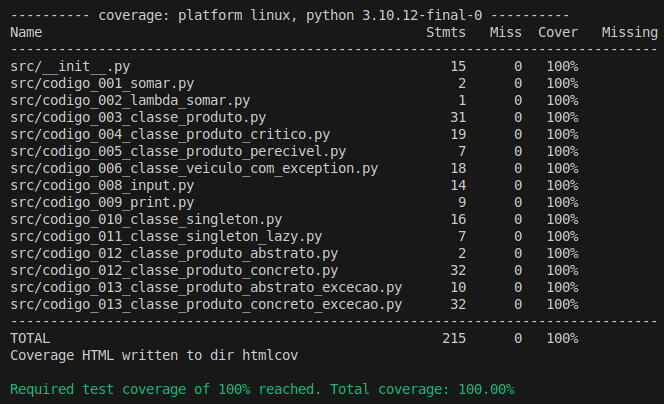
\includegraphics[scale=0.4]{imagens/fig-result-test-produto-concreto.png}
	
	\vspace{0.25em}
	\fontsize{9pt}{10}\selectfont{
		*obs: \textit{pytest --maxfail=1  --cov-fail-under=100 --disable-warnings --cov=./src --cov-report=html --cov-report=term-missing}
	}\par
	
\end{frame}






\begin{frame}[t]{Interface com Classes Abstratas - Caso com Exceção}
	
	%	\lstinputlisting[style=CBruno,caption=Classe Produto Abstrato Excecao]{outros/codigos/python/exemplos-de-aulas/src/codigo_013_classe_produto_abstrato_excecao.py}
	
	\centering
	\makebox[\linewidth][c]{
		\begin{minipage}{0.95\textwidth}
			\inputminted[baselinestretch=1,fontsize={\fontsize{8}{8}\selectfont}]{python}{outros/codigos/python/exemplos-de-aulas/src/codigo_013_classe_produto_abstrato_excecao.py}
		\end{minipage}
	}
	\fontsize{7pt}{6}\selectfont{
		Classe Produto Abstrato Exceção - codigo\_013\_classe\_produto\_abstrato\_excecao.py
	}\par
	
	
\end{frame}

\begin{frame}[t]{Interface com Classes Abstratas - Caso com Exceção}
	\vspace{-0.5em}
	%	\lstinputlisting[style=CBruno,caption=Classe Produto Concreto Excecao]{outros/codigos/python/exemplos-de-aulas/src/codigo_013_classe_produto_concreto_excecao.py}
	\centering
	\makebox[\linewidth][c]{
		\begin{minipage}{0.95\textwidth}
			\inputminted[fontsize={\fontsize{6}{6}\selectfont}]{python}{outros/codigos/python/exemplos-de-aulas/src/codigo_013_classe_produto_concreto_excecao.py}
		\end{minipage}
	}
	\fontsize{7pt}{6}\selectfont{
		Classe Produto Concreto Exceção - codigo\_013\_classe\_produto\_abstrato\_excecao.py
	}\par
\end{frame}


\begin{frame}[t]{Teste Unitário}
	
	%	\vspace{-1em}
	%	\lstinputlisting[style=CBruno,caption=Cobertura de testes da classe Produto Concreto Exceção]{outros/codigos/python/exemplos-de-aulas/tests/test_codigo_013_classe_produto_concreto_excecao.py}
	
	\centering
	\makebox[\linewidth][c]{
		\begin{minipage}{0.95\textwidth}
			\inputminted[baselinestretch=1,fontsize={\fontsize{9}{8}\selectfont}]{python}{outros/codigos/python/exemplos-de-aulas/tests/test_codigo_013_classe_produto_concreto_excecao.py}
		\end{minipage}
	}
	\fontsize{7pt}{6}\selectfont{
		Cobertura de testes da classe Produto Concreto Exceção - test\_codigo\_013\_classe\_produto\_concreto\_excecao.py
	}\par
	
\end{frame}








\begin{frame}[t]{Tratamento de exceções}
	
	\fontsize{13pt}{15}\selectfont{
		
		O tratamento de exceção, na ciência da computação, é o mecanismo responsável pelo tratamento da ocorrência de condições que alteram o fluxo normal da execução de programas de computadores. \\
		\vspace{0.5em}
		Para condições consideradas parte do fluxo normal de execução, ver os conceitos de sinal e evento.
		
	}\par
	
	\vspace{2em}
	Saiba mais em\\
	\fontsize{10pt}{15}\selectfont{
		\url{https://docs.python.org/pt-br/3/whatsnew/2.6.html\#pep-3110-exception-handling-changes}\\
		\url{https://docs.python.org/pt-br/3/reference/compound_stmts.html\#except-clause}\\
		\url{https://docs.pytest.org/en/stable/how-to/assert.html}
	}\par
\end{frame}


\begin{frame}[t]{Tratamento de exceções}
	
	\vspace{1em}
	
	\fontsize{13pt}{15}\selectfont{
		A sintaxe básica é:
	}\par
	
	\vspace{1em}
	\begin{beamercolorbox}[wd=\textwidth]{warning}
		try: \\
		\hspace{1em}{Instruções} \# o código da funcionalidade.\\
		...\\
		except <ExceptType>:\\
		\hspace{1em}{Instruções} \# o código para tratamento da exceção.\\
		...\\
		finally: \# Caso o fluxo não seja interrompido, sempre é executado o finally.\\
		\hspace{1em}{Instruções}
	\end{beamercolorbox}
	
	
	\vspace{2em}
	\url{https://docs.python.org/pt-br/3/tutorial/errors.html}
	
\end{frame}


\begin{frame}[t]{Tratamento de exceções}
	
	\lstinputlisting[style=CBruno,caption=Tratamento de exceções]{outros/codigos/python/exemplos-de-aulas/src/codigo_006_classe_veiculo_com_exception.py}
	
	
\end{frame}


\begin{frame}[t]{Pytest}
	
	%	\vspace{-2em}
	\lstinputlisting[style=CBruno,caption=Cobertura de testes da classe Veiculo]{outros/codigos/python/exemplos-de-aulas/tests/test_codigo_006_classe_veiculo_com_exception.py}
	
	
\end{frame}














\begin{frame}[t]{Polimorfismo em classe}
	
	\fontsize{14pt}{15}\selectfont{
		
		Polimorfismo permite que objetos de diferentes classes sejam tratados como objetos de uma classe comum.
		
	}\par
	\vspace{1em}
	
	\fontsize{12pt}{15}\selectfont{
		\begin{itemize}%[<+->] 
			
			\item Polimorfismo é o princípio pelo qual duas ou mais classes derivadas de uma mesma superclasse podem invocar métodos que têm a mesma identificação, assinatura, mas comportamentos distintos, especializados para cada classe derivada, usando para tanto uma referência a um objeto do tipo da superclasse.
			
			%			\item 
			
		\end{itemize}
	}\par
	\vspace{1em}
	
\end{frame}






\begin{frame}[t]{Polimorfismo em classe}	
	
	\lstinputlisting[style=CBruno,caption=Polimorfismo de classe]{outros/codigos/python/exemplos-de-aulas/src/codigo_005_classe_produto_perecivel.py}
	
	\vspace{1em}
	
	*obs: \textbf{class ProdutoPerecivel(Produto)} é uma classe derivada de Produto: indica que \textbf{ProdutoPerecivel} é uma subclasse da classe \textbf{Produto}.
	
\end{frame}

\begin{frame}[t]{Pytest}
	
	%	\vspace{-2em}
	\lstinputlisting[style=CBruno,caption=Cobertura de testes da classe Produto Perecivel]{outros/codigos/python/exemplos-de-aulas/tests/test_codigo_005_classe_produto_perecivel.py}
	
	
\end{frame}




\begin{frame}[t]{Pytest}
	
	\centering
	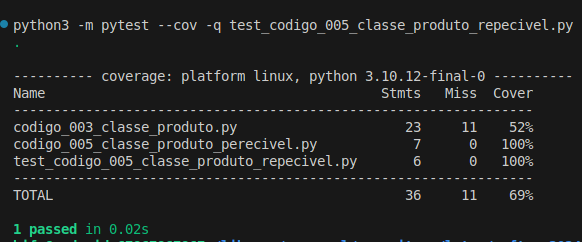
\includegraphics[scale=0.5]{imagens/fig-result-test-especifico-produto-perecivel.png}
	
\end{frame}


\begin{frame}[t]{Pytest}
	
	\centering
	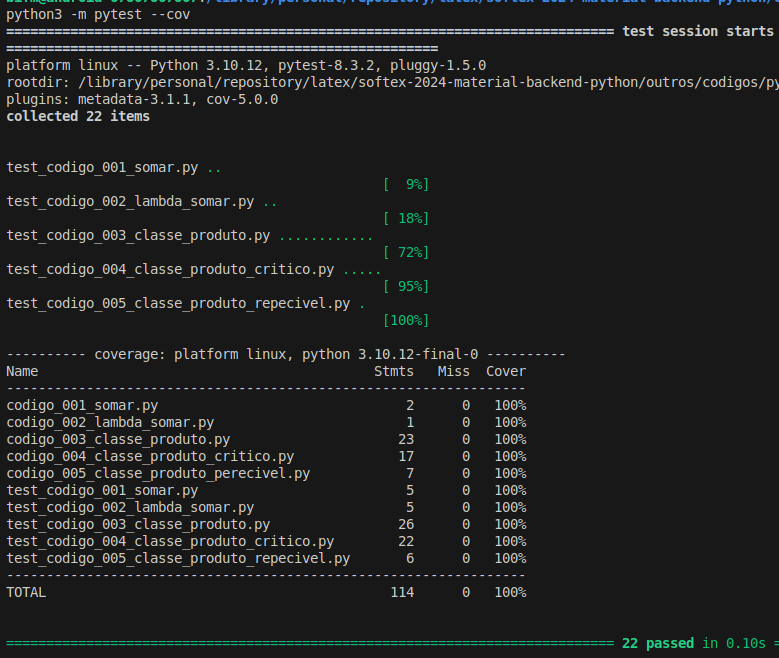
\includegraphics[scale=0.3]{imagens/fig-result-test-produto-perecivel.png}
	
\end{frame}






\begin{frame}[t]{Polimorfismo em classe}	
	
	\fontsize{14pt}{15}\selectfont{
		
		Sobreposição.
		
	}\par
	\vspace{1em}
	
	\fontsize{12pt}{15}\selectfont{
		\begin{itemize}%[<+->] 
			
			%			\item Sobrecarga (Overload): é o ato de criar vários métodos diferentes com o mesmo o nome, porém com assinaturas diferentes, cada um com sua própria implementação. Python não trabalha com overload por padrão. Para alcançar é possível utilizar bibliotecas com decoratores.
			
			\item Sobreposição (Override): é sobrescrever, ou seja, definir um novo comportamento para um método que já existe. Isso acontece quando a classe em questão herda (estende) outra classe e se cria um método com a mesma assinatura da classe "pai" na classe filha.
			
		\end{itemize}
	}\par
	\vspace{1em}
	
\end{frame}



\begin{frame}[t]{Encapsulamento em classe}
	
	\fontsize{12pt}{15}\selectfont{
		
		Encapsulamento é a proteção dos atributos ou métodos de uma classe, em Python existem somente o public e o private e eles são definidos no próprio nome do atributo ou método.
		
	}\par
	
	\vspace{0.5em}
	\fontsize{8pt}{10}\selectfont{
		\begin{beamercolorbox}[wd=\textwidth]{warning}
			class Veiculo:\\
			\hspace{1em}chassi = 1 \# atributo publico\\
			\hspace{1em}\_\_motor = 2 \# atributo privado a classe Veiculo. O símbolo \_\_* define como privado.\\
			\vspace{0.5em}
			class Carro(Veiculo):\\
			\hspace{1em}\_\_placa = 3 \# atributo privado a classe Carro\\
			\vspace{0.5em}
			\hspace{1em}def \_\_init\_\_(self):\\
			\hspace{2em}print(self.chassi)\\
			\hspace{2em}print(self.\_\_placa)\\
			\vspace{0.5em}
			veiculo = Veiculo()\\
			print(veiculo.chassi) \# imprime 1\\
			\vspace{0.5em}
			carro = Carro() \# Erro\\
			\# print(carro.\_\_motor) \# Erro, pois \_\_motor é privado a classe Veiculo.\\
			\# print(carro.\_\_placa) \# Erro, \_\_placa é um atributo privado, somente chamado pela classe Carro.\\
		\end{beamercolorbox}
		
	}\par
	\vspace{1em}
	
	
\end{frame}






\begin{frame}[t]{Encapsulamento em classe}
	
	\begin{block}{Exemplo anteior}		
		class Veiculo:\\
		\hspace{1em}chassi = 1 \# atributo publico\\
		\hspace{1em}\_\_motor = 2 \# atributo privado a classe Veiculo. O símbolo \_\_* define como privado.\\
		\vspace{0.5em}
		class Carro(Veiculo):\\
		\hspace{1em}\_\_placa = 3 \# atributo privado a classe Carro\\
		\vspace{0.5em}
		\hspace{1em}def \_\_init\_\_(self):\\
		\hspace{2em}print(self.chassi)\\
		\hspace{2em}print(self.\_\_placa)\\
		\vspace{0.5em}
		veiculo = Veiculo()\\
		print(veiculo.chassi) \# imprime 1\\
		\vspace{0.5em}
		carro = Carro() \# Erro\\
		\# print(carro.\_\_motor) \# Erro, pois \_\_motor é privado a classe Veiculo.\\
		\# print(carro.\_\_placa) \# Erro, \_\_placa é um atributo privado, somente chamado pela classe Carro.\\
	\end{block}
	
	
\end{frame}





